\section{Banc de registres}

\subsection{Description}

\subsection{Interface}

\subsubsection{Entrées}

\begin{tabular}{|l|r|l|}
\hline
\textbf{Port}		& \textbf{Taille} & \textbf{Description}\\
\hline

\texttt{DataIn}		& \texttt{32} & Données entrantes, à enregistrer dans le registre sélectionné\\
\hline
\texttt{RegDest}	&  \texttt{3} & Sélection du registre de destination des données entrantes\\
\hline
\texttt{Clk}		&  \texttt{1} & Horloge\\
\hline
\texttt{Reset}		&  \texttt{1} & Remise à zéro\\
\hline
\texttt{RegA}		&  \texttt{3} & Sélection du registre A pour les données sortantes\\
\hline
\texttt{RegB}		&  \texttt{3} & Sélection du registre B pour les données sortantes\\

\hline
\end{tabular}


\subsubsection{Sorties}

\begin{tabular}{|l|r|l|}
\hline 
\textbf{Port} & \textbf{Taille} & \textbf{Description}\\
\hline

\texttt{AOut}	& \texttt{32} & Données sortantes du registre sélectionné A\\
\hline
\texttt{BOut}	& \texttt{32} & Données sortantes du registre sélectionné B\\
\hline
\texttt{R0}	& \texttt{32} & Registre interne 0\\
\hline
\texttt{R1}	& \texttt{32} & Registre interne 1\\
\hline
\texttt{R2}	& \texttt{32} & Registre interne 2\\
\hline
\texttt{R3}	& \texttt{32} & Registre interne 3\\
\hline
\texttt{R4}	& \texttt{32} & Registre interne 4\\
\hline
\texttt{R5}	& \texttt{32} & Registre interne 5\\
\hline
\texttt{R6}	& \texttt{32} & Registre interne 6\\
\hline
\texttt{R7}	& \texttt{32} & Registre interne 7\\

\hline
\end{tabular}

Les sorties \texttt{R0-R7} ne seront pas utilisées pour implémenter une quelconque fonctionalité. Elles sont présentes pour aider à visualiser le comportement du processeur.

\subsection{Interaction avec l'ALU}

Après avoir réalisé l'ALU et le banc de registres, l'interaction entre ces composants peut être mise en oeuvre de la manière suivante:

\hspace{14em}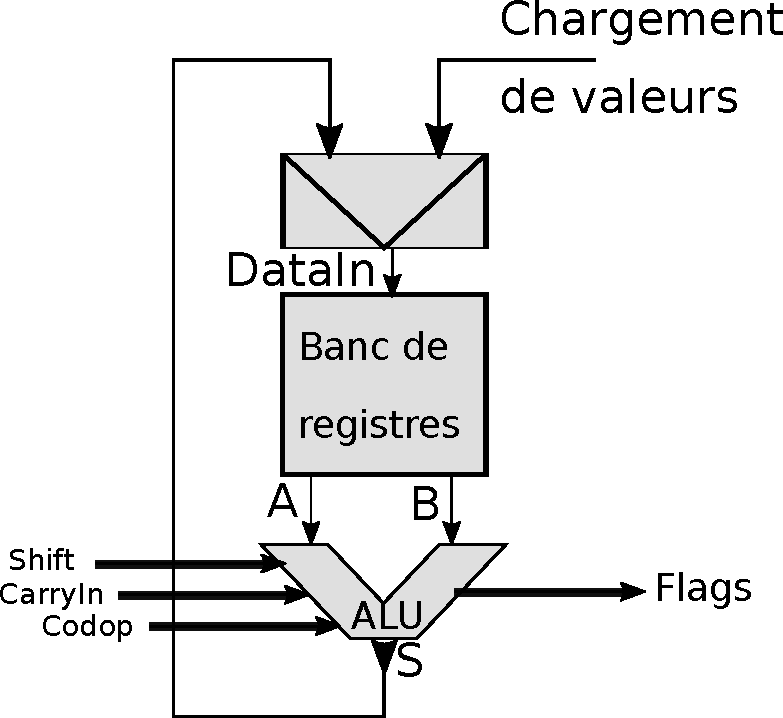
\includegraphics[scale=0.5]{pictures/ALU_Registers.pdf}

Il est ainsi possible de valider leur comportement en enregistrant des données dans le banc de registre (à l'aide des ports \texttt{DataIn} et \texttt{RegDest})
puis en effectuant diverses opération par l'ALU en spécifiant  le \texttt{Codop}.
